\documentclass[sigconf, nonacm]{acmart}
\usepackage{hyperref}
\usepackage{todo}
\usepackage[outputdir=.texpadtmp]{minted}

\settopmatter{printacmref=false}
\renewcommand\footnotetextcopyrightpermission[1]{} % removes footnote with conference info

\setcopyright{none}

\setlength{\parskip}{6px} 

\begin{document}
\title{AirSense - a personal air quality monitoring device}
\subtitle{IoTSSC Coursework Report}

%%
%% The "author" command and its associated commands are used to define
%% the authors and their affiliations.
%% Of note is the shared affiliation of the first two authors, and the
%% "authornote" and "authornotemark" commands
%% used to denote shared contribution to the research.
\author{Robert Phipps}
\authornote{This was a joint project with Kyle Cooke s1511964, but this report 
is individual work.}
\email{s1601921@ed.ac.uk}
\affiliation{%
  \institution{University of Edinburgh Informatics}
}

%%
%% This command processes the author and affiliation and title
%% information and builds the first part of the formatted document.
\maketitle

\section{Project overview}

AirSense is an IoT solution to allow individuals to track their own exposure to air
pollution, and enable them to make informed changes to improve their personal health.

The system makes use of a Bluetooth Classic (2.1) sensor pack, that can be attached to a bag, 
which periodically reads air quality data using a variety of sensors. This data is pushed to 
a companion app running on the user's phone, which calculates an air quality metric. This
data is then uploaded to the AirSense cloud (operating on Google Firebase), to allow a 
global map of anonymised air quality data to be built.

\subsection{Example Use Case and User Story}

To allow development to reasonably focussed on a realistic scenario, this is our example
use case:

\begin{quotation}
	"The user is a worker with no fixed office, so is working in uncontrolled environments
	in multiple locations throughout the day. At the end of the day, they like to go 
	cycling. They are sensitive to pollution and their family has a history of Asthma, so
	they are keen to minimise their exposure to poor air quality. They also have some 
	favourite locations that they regularly visit, and would like to know before they leave
	if those locations are struggling with high pollution.
	
	In the morning, they unplug their air sensor unit from charge, clip it to their rucksack,
	and leave for work. Throughout the day they work as normal, and allow the sensor to 
	record their exposure to pollution. As they are about to leave for the Meadows to eat
	their lunch, they receive a notification to say pollution there is high today, so they
	opt to eat inside.
	
	When they get home, they check to see their daily exposure, and then check the global
	heatmap to identify a location with low pollution where they can go for their evening
	cycle.
	
	As a way to incentivise themselves to take action to reduce their exposure, they have
	entered into a competition with friends, and will use their leaderboard score to work
	out who is doing best."
\end{quotation}

\subsection{Implementation problems}

When designing a system such as this, with multiple moving parts across different platforms,
and acquisition of data from sensors, there are several issues that need to be addressed:

\begin{itemize}
	\item What data to we want to record from the air sensors?
	\item How are we getting that data to the cloud storage?
	\item How do we represent the data in a reasonable and understandable way?
	\item How do we ensure minimal performance impact/reasonable battery life?
	\item What infrastructure do we use to ensure maintainability and scalability?
\end{itemize}

We believe we have found reasonable answers to these problems, which are detailed in this
report.

\subsection{Existing products on the market}

In terms of existing, commercially available products which perform personal air quality
monitoring, there are remarkably few, given the proliferation of health-tracking related
gadgets appearing on the market currently.

Plume Labs has their "Flow 2" product available for £139, which seems to cover a lot of the
features we are targeting with AirSense, although it makes use of Bluetooth Low Energy and
has additional sensors for PM1 and PM10. They also have developed a custom "neural engine" 
to calculate their air quality metric, with help from researchers at Imperial College London.
It claims to have a typical battery life of 24-72 hours.

\section{Creating an Air Quality Metric}

\subsection{Sensors available}

As part of this project, we were given hardware capable of sensing the following airborne
chemical compounds and particles:

\begin{itemize}
	\item Optical dust sensor: PM2.5 particulate matter
	\item Grove multichannel gas sensor v1.0: \cite{grove_sensor}
		\begin{itemize}
			\item Carbon Monoxide
			\item Nitrogen Dioxide (NO2)
			\item Ethanol
			\item Hydrogen
			\item Ammonia
			\item Methane, Propane, Iso-butane
		\end{itemize}
	\item Adafruit SGP30 gas sensor \cite{lady_ada_adafruit_2019}
		\begin{itemize}
			\item Total Volatile Organic Compounds (tVOC)
			\item Equivalent CO2 (eC02)
		\end{itemize}
\end{itemize}

This is a fairly large volume of data that we have available to us\cite{wiki_aqi}, although just presenting
these raw values to the user is unlikely to be very helpful at all. We needed to find a way to 
combine all of these sensor readings into a single, simple to understand metric.

\subsection{Existing metrics}

Unsurprisingly, we aren't the first people to have encountered this issue. There are multiple
air quality metrics already in existence, used by environmental institutions all across the world.

\textbf{The UK's Daily Air Quality Index (DAQI)} \cite{defra_aqi}

This index is used by the UK Department for Environment, Food \& Rural Affairs, is based on a 1-10
scale, and uses five pollutants in its calculation. It was recommended by the Committee on Medical 
Effects of Air Pollutants, and is the index shown in UK weather forecasts.

It uses NO2, S02, O3, PM2.5 and PM10, however with our sensors, we are only able to measure
two of those five pollutants (NOx and PM2.5), so this index was ruled out.

\textbf{The European Air Quality Index} \cite{euro_aqi}

This system was co-developed by the European Commission's Directorate General for Environment and
the European Environment Agency. It uses the same components as the DAQI, and takes the worst score 
for any of the pollutants as the overall score. It is heavily weighted towards PM2.5.

Unfortunately, again, we don't have the sensors to accurately use this system for our AQI.

\textbf{The United States EPA's Air Quality Index} \cite{airnow_aqi}

This system was developed by the US Environmental Protection Agency, and uses a combination of
O3, PM2.5, PM10, CO, SO2 and NO2 to calculate its score. Unfortunately we don't have all of these
sensors, however we are able to achieve a rough approximation using the PM2.5, CO and NO2 readings.

\subsection{Our metric}

We have opted to base our metric off of the EPA's AQI, as this gives us a very firm base to work on,
and allowing readings from AirSense to be used along with readings from external measuring stations.

The metric is calculated on the Android app, using the breakpoints defined by the EPA shown in figure
\ref{fig:aqicalc}.

\section{Hardware design}

\subsection{Development platform}

For this project, the NXP FRDM-K64F embedded development platform forms the base of the
hardware solution, running Mbed OS. \cite{frdm_k64f}

It is paired with a number of outboard devices, to provide both communication and sensing.
Figure \ref{fig:hardwareschem} is a very high-level overview of how these devices are connected together.

\begin{figure}[h]
	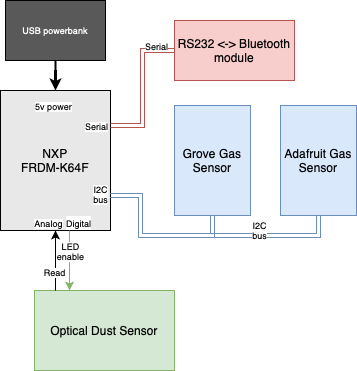
\includegraphics[width=0.8\columnwidth]{hardware-schem.png}
	\caption{Overview schematic of hardware modules}
	\label{fig:hardwareschem}
\end{figure}

All power for this solution currently comes from a 5v USB power bank. This is a high-capacity
lithium battery, with integrated charging and protection circuitry. We are also using the
3.3v regulator within the FRDM board to provide level shifted power for components that require 
it, although in later revisions this should likely be offloaded to a dedicated power management
module, which would be required for management of a "naked" lithium cell in any case.

There are no controls on the development board, as all commands are sent via the Bluetooth/
serial link. Pairing is automatically initiated with the Bluetooth module whenever there is
no device connected.

Several modules (for example the Grove gas sensor) are comparatively high power consumption, 
with integrated heating elements. It was investigated as to whether we could completely cut
power to these when they are not in use (in between readings), however they experienced issues
re-establishing communication with the I2C bus, causing Mbed OS to crash. As such there are
methods implemented within firmware to reduce power consumption where possible.

\subsection{Device firmware}

\begin{figure*}
	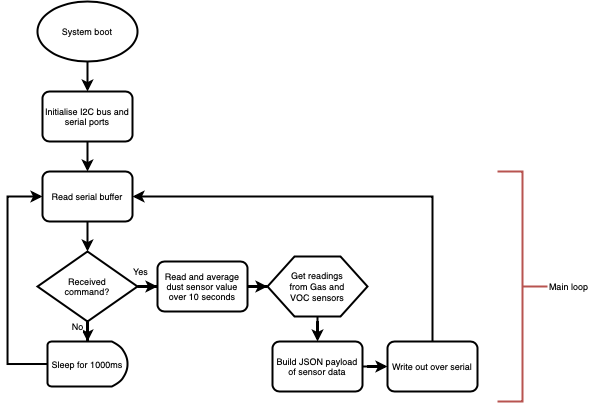
\includegraphics[width=0.8\textwidth]{firmware-flow}
	\caption{Flowchart of main firmware functions}
	\label{fig:firmwareflow}
\end{figure*}

As this platform runs Mbed OS, the firmware is written as C++, and takes advantage of the 
multithreading and sleep states available within the operating system.

To reduce power consumption, the board is configured to enter a sleep state in between polls
of the serial buffer. It will only power on and read from the sensors if a request has been
made to through the serial communications. The app is configured to only request an update 
every 60 seconds, so this means the board is idle for a lot of the time. Based on the Mbed OS 
profiling tools, the board was in these sleep states 96\% of the time.

The basic process chart is shown in figure \ref{fig:firmwareflow}.

Due to the dust sensor having incredibly unstable readings, the FRDM board takes an average of
30 readings over 3 seconds. There is still some considerable variation, but this improves 
things greatly.

This firmware is completely stateless, so the hardware module can be rebooted at any time
without data loss, as all data is streamed directly to the app. This does mean that if
Bluetooth communication with the app is interrupted, sensor readings will not be taken,
however as AirSense is designed to monitor the quality of the air around a person and not
at a fixed location, and uses the phone's GPS to tag those locations, this is not a problem. 
If the hardware board were to cache readings and bulk upload them to the app, we would first
have no idea where these readings were taken, nor an accurate time of acquisition, as the 
FRDM platform does not include a battery backed real time clock.

\subsection{Enclosure}

We also designed a custom enclosure (figure \ref{fig:casing}) for the solution and all sensors, to be manufactured
with CNC (either cut from sheet material, or 3D printed). We were unable to bring this
design to life as the uCreate Studio shut before we could get any time on the machines.

\begin{figure}
	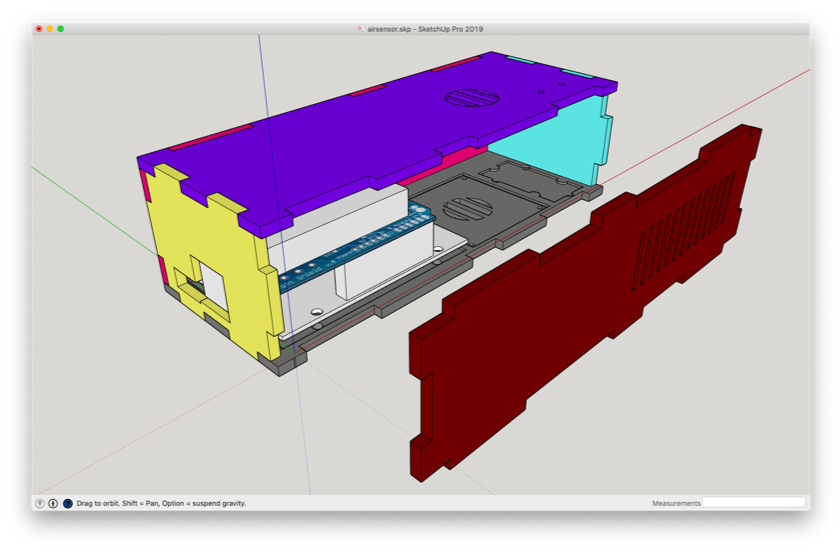
\includegraphics[width=\columnwidth]{casing}
	\caption{3D model of casing design}
	\label{fig:casing}
\end{figure}

\section{Android app}

\subsection{User interface}

The app has a fairly minimal user interface, with only those features that are required to
get up and running with AirSense. 

Beyond the initial setup wizard, functionality within the app is limited to viewing of current
exposure score and configuration of alert subscriptions. All data visualisation is possible
through the mobile-friendly web-app. This approach was adopted as after investigating data-
visualisation options within the Android platform, we decided that there simply wasn't enough
screen space on a mobile device to create a comfortable way to display the information.

Ultimately, the first and foremost function of the app is configure the background DataLogger
service.

\subsection{Authentication to cloud}

To make authentication incredibly simple, we use the Firebase Auth library\cite{firebase_auth}, and the associated
Firebase UI package. This offers a drop-in, turnkey solution for user authentication, following
all best practices, and allowing us to enable support for various authentication providers
such as Google, Facebook, phone, email and many other OAuth capable services.

This library automatically authenticates future communications to Firebase services such as 
the Firestore cloud database while the user is signed in.

\subsection{Alert push notifications}

To allow the user to receive push notifications in response to alert subscriptions they have
set up, we make use of the Firebase Cloud Messaging service\cite{firebase_messaging} . This provides a simple wrapper
for the Google push messaging API. This runs as another service on the phone, and provides
a very simple way to push these alerts down from the cloud platform.

\subsection{IoT gateway functionality (DataLogger service)}

In this solution, the Android app (companion app) acts as the gateway to allow data from the
hardware device to be written into the AirSense cloud platform.

The app incorporates a foreground service within Android, which allows it to continually run
even with the phone in sleep mode or when the user is using other apps. This service includes
a timer to periodically (every one minute), request a sensor update JSON package from the 
hardware device over Bluetooth, before reformatting that package, adding location data and 
calculating the Air Quality Index and uploading that data to the cloud database backing
the AirSense service.

This method was chosen as firstly by using the phone as the cellular modem and GPS module, 
far less hardware needed to be incorporated as part of the sensor pack. It also means that
there are no additional fees associated with using AirSense (as opposed to cellular SIM card
rental), and reduces power consumption of the hardware device considerably.

In this setup, the phone requests the sensor readings from the sensor when it is ready, as 
opposed to subscribing to periodic updates from the hardware device. This method ensures that
the sensors are only read when the phone is ready to receive and process an update, for 
example once the user is signed in and Bluetooth has been paired.

All communication with the cloud database is managed with the native Firebase Firestore 
libraries.\cite{firebase_firestore}

\begin{figure*}
\begin{minted}{kotlin}
fun messageToAQI(message: SerialMessage): Float? {
  val co = interpolateBetweenBreaks(message.co,4.4f, 9.4f, 12.4f, 15.4f, 30.4f, 40.4f, 50.4f)
  val no2 = interpolateBetweenBreaks(message.no2, 53f,100f,360f,649f,1249f,1649f,2049f)
  val dust = interpolateBetweenBreaks(message.dust?.times(1000), 35000f,75000f,115000f,150000f,
                 250000f,500000f, 750000f)
  return max(max(co!!, no2!!), dust!!)
}
\end{minted}
\caption{Calculating AQI from the three raw sensor values in Kotlin}
\label{fig:aqicalc}
\end{figure*}

\subsection{Optimising resource usage}

As this app is running on a multi-purpose device, we needed to ensure that we were considerate
with the app's resource usage. The scheduled updates (every 60 seconds) make use of a 
\texttt{TimerTask} within Android, which allows the majority of the app to be suspended
outside of the occasional update tasks.

We also only perform minimal data massaging within the app, being some reformatting and 
calculation of the AQI (some basic arithmetic). This means that the service only has to
write a single document to the cloud database. All other data management tasks are carried
out in the cloud.

If internet connection fails on the phone, the Firebase libraries handle queuing of readings,
which are then uploaded once the phone comes online again.

The Android \texttt{FusedLocationProvider()}\cite{android_fusedlocation} is used to access fine location of the phone
to geotag sensor readings, however this is only polled on a sensor update (once every 60 
seconds). This provider automatically makes use of the best location provider available, so
in the event that the Google Location Service has been able to use nearby wireless networks
to locate the phone, that data will automatically be used. This method should reduce the amount
of time the GPS module within the phone is active, and also battery usage.

\begin{table*}[p]
\begin{tabular}{@{}lp{0.24\textwidth}l@{}}
\toprule
\textbf{Collection}              & \textbf{Purpose}                                                            & \textbf{Document schema}                                                                                                                                                                                                                                                               \\ \midrule
georeadings             & Air quality reading for a specific location - 1 entry per location & \begin{tabular}[c]{@{}l@{}}{[}random id{]}: \{\\\hspace{6pt}l: location coordinates\\\hspace{6pt}g: geocode hash\\\hspace{6pt}d: \{\\\hspace{12pt}basedOn: number of readings\\\hspace{12pt}score: air quality score\\\hspace{6pt}\}\\\} {[}...{]}\end{tabular}                                                                \\ \midrule
readings                & Individual air quality readings - multiple readings per location   & \begin{tabular}[c]{@{}l@{}}{[}random id{]}: \{\\\hspace{6pt}aqi: calculated air quality score\\\hspace{6pt}auth: user ID\\\hspace{6pt}c2h5oh: raw sensor reading\\\hspace{6pt}{[}...{]} \\\hspace{6pt}h2: raw sensor reading\\\hspace{6pt}l: location\\\hspace{6pt}t: timestamp\\ \} {[}...{]}\end{tabular}                                \\ \midrule
userexposure            & Per user pollution exposure scores, per day and rolling average    & \begin{tabular}[c]{@{}l@{}}{[}date{]}: \{\\\hspace{6pt}exposureTotal: score\\ \}\\ {[}date{]}: \{\\\hspace{6pt}exposureTotal: score\\ \}\\ {[}...{]}\\ d: \{\\\hspace{6pt}basedOn: number of readings\\\hspace{6pt}score: rolling average score\\ \}\end{tabular}                                                 \\ \midrule
userscores              & Leaderboard data                                                   & \begin{tabular}[c]{@{}l@{}}{[}date{]}: \{\\\hspace{6pt}scores: \{\\\hspace{12pt}{[}userid{]}: \{\\\hspace{18pt}name: username,\\\hspace{18pt}score: leaderboard score\\\hspace{12pt}\}\\\hspace{6pt}\}\\ \} {[}...{]}\end{tabular}                                                                                        \\ \midrule
notificationSubscribers & Alert subscriptions (GeoFirestore Geopoint)                        & \begin{tabular}[c]{@{}l@{}}{[}random id{]}: \{\\\hspace{6pt}d: \{\\\hspace{12pt}auth: user id\\\hspace{12pt}coordinates: location\\\hspace{12pt}limit: radius\\\hspace{12pt}name: user defined name\\\hspace{12pt}registrationToken: messaging token\\\hspace{6pt}\}\\\hspace{6pt}g: geohash\\\hspace{6pt}l: location\\ \} {[}...{]}\end{tabular} \\ \bottomrule
\end{tabular}
\caption{Firestore collections}
\label{tab:firestore}
\end{table*}

\section{Cloud infrastructure}

\subsection{Overview}

All cloud services are powered by Google's Firebase platform. Firebase is designed as a way to
quickly bootstrap apps and services, within a fully managed and incredibly scalable 
environment. Firebase was chosen because of it's very deep integration with Android, 
fantastic libraries, integrated authentication and the ability for it to be used within
the Google Cloud Platform environment we were given access to.

\subsection{Database (Firestore)}

Firestore is a NoSQL database system, which we use for storing readings from clients, user
scores and the global store of air quality readings. The database collections are defined in
table \ref{tab:firestore}.

Firestore (unlike Google BigQuery) has incredibly minimal support for GIS style queries, which
was going to be a problem for us, as we need to be able to efficiently query for documents
around a point within a certain radius. To allow us to have this functionality, we are making
use of the GeoFirestore library. This creates hashes and adds this functionality on top of the
existing Firebase featureset. It isn't as efficient as BigQuery's implementation, however it does
enough, and allows us to remain entirely within the Firebase ecosystem.

There are also a couple of Firebase Cloud Functions\cite{firebase_functions} which are used to to manage data in this
system. The first is exposed as an API endpoint. This endpoint is used by the heatmap within
the web app as it generates a GeoJSON document containing \texttt{georeading} datapoints within
a requested area.

The second is registered to run every time a document is added to the \texttt{readings} collection
by an instance of the Android app. This performs the actions shown in figure \ref{fig:cloudfunctions}.

\begin{figure*}[h]
	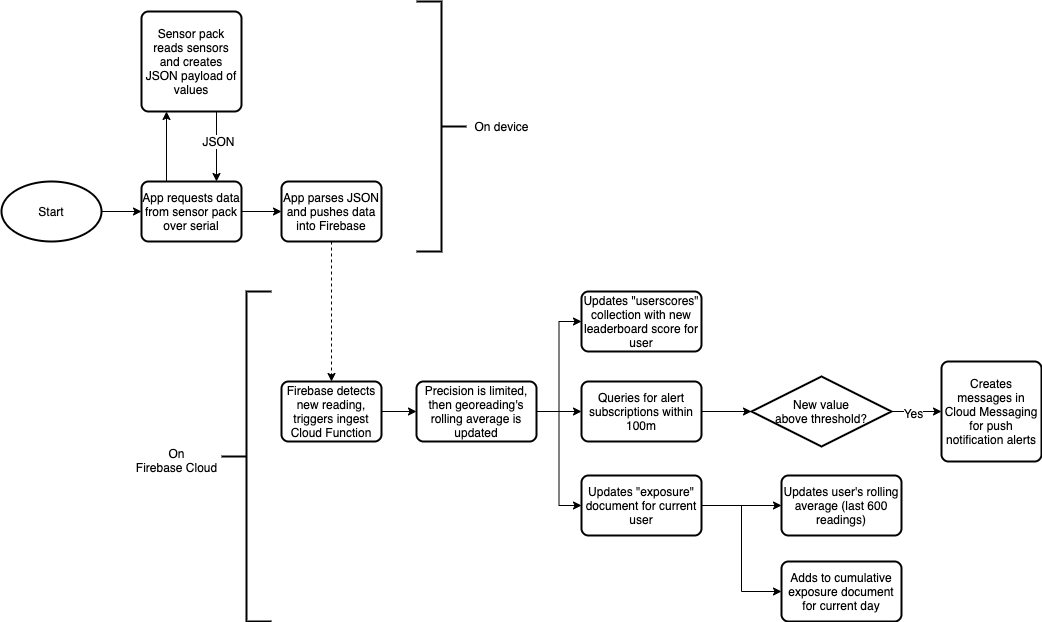
\includegraphics[width=0.9\textwidth]{cloudfunctions}
	\label{fig:cloudfunctions}
	\caption{Cloud functions on receipt of new reading}
\end{figure*}

It is worth specifically noting that the \texttt{georeading} documents used by the app as the 
global air quality scores for the heatmap are generated by this cloud function and not by the
app. As part of this, we round the latitude and longitude to 0.005 decimal places to ensure
a fixed density of datapoints, and calculate a rolling average based off any previous readings
to ensure that single erroneous readings do not cause too much problem to the wider dataset.

\subsection{Push notifications (Cloud Messaging)}

To enable support for push notifications in response to air quality alerts, we are using a fairly basic 
implementation of Firebase Cloud Messaging\cite{firebase_messaging}. This allows users to very easily register to receive alerts,
which creates an entry in Firestore's \texttt{notificationSubscribers} collection. The data ingest Cloud
Function checks for any nearby alerts when a new reading hits the database, and uses the 
\texttt{registrationToken} with the Cloud Messaging client to send a push notification to the service
running within the app.

\begin{figure*}[p]
	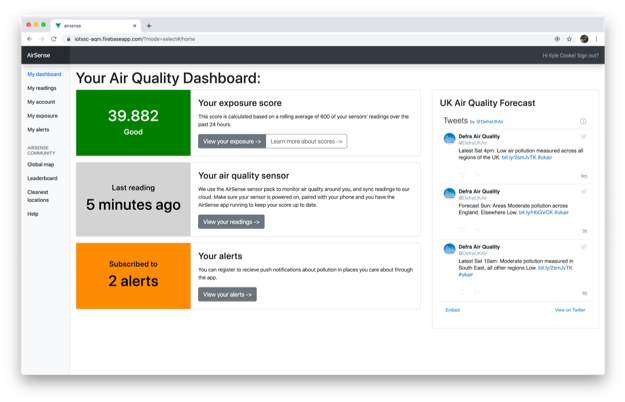
\includegraphics[width=0.7\textwidth]{webapp-1}
	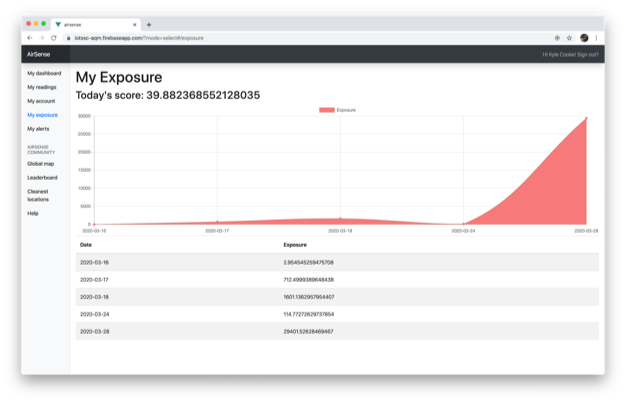
\includegraphics[width=0.7\textwidth]{webapp-2}
	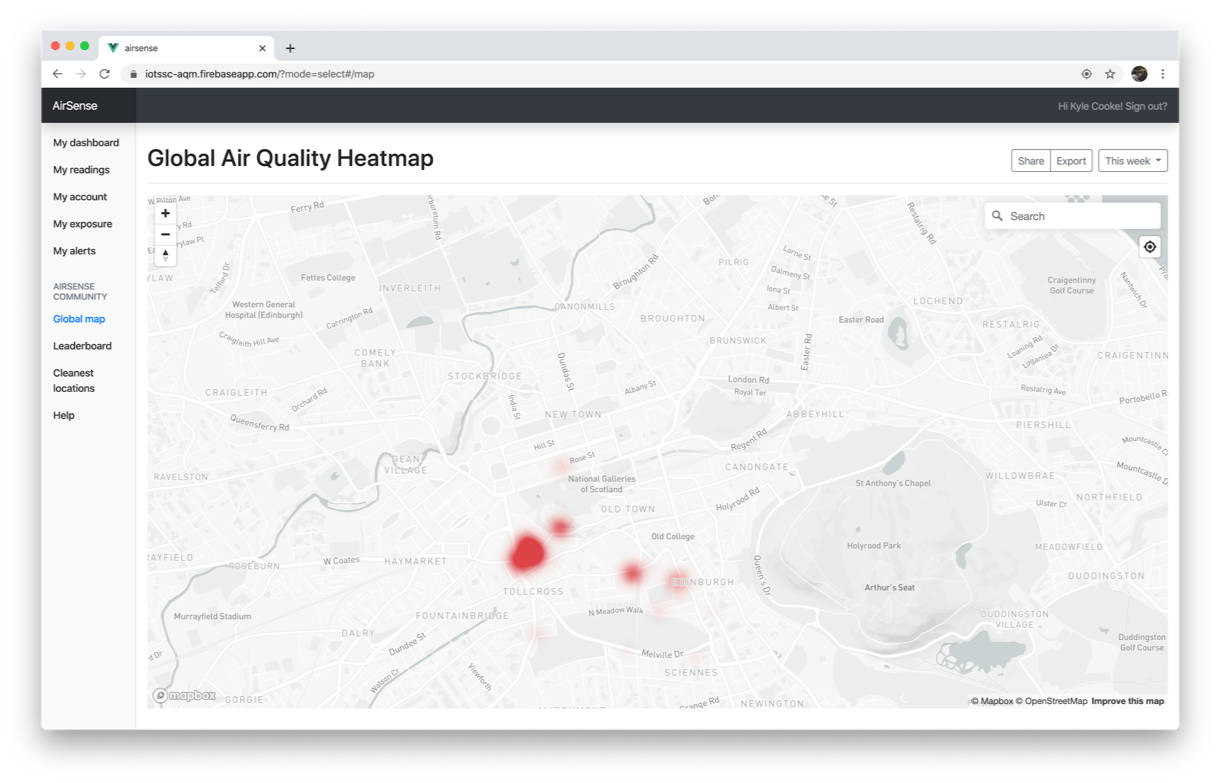
\includegraphics[width=0.7\textwidth]{webapp-3}
	\caption{Screenshots of the AirSense web app}
	\label{fig:webapp}
\end{figure*}

\subsection{Web app}

The main way users interact with AirSense is via the web app. (Figure \ref{fig:webapp}) This includes multiple data visualisations,
including a global heatmap, historical exposure graphs and colour coded exposure scores. There is also
alert subscription management and the ability to view raw sensor data uploaded to the cloud. We have
also implemented a leaderboard, which would show the user who has the most low-pollution readings in the
last day.

The web app is developed as a single page Vue.js\cite{vuejs_home} app, with Bootstrap for UI elements and responsive 
features. It is hosted within Firebase on their Hosting service\cite{firebase_hosting}. Data is pulled in using the Firebase
Firestore JavaScript libraries, and the drop-in Firebase Auth authentication flow is used to handle
logins and signups.

The heatmap representation is powered by MapBox GL JS\cite{mapbox_intro}, and pulls in a GeoJSON of data (centered and
limited around the map viewport), which is loaded into a data layer. The visualisation is not ideal,
as it only shows areas we know have pollution. Areas that have no data or have no pollution are both
displayed in the same way (no overlay). We looked into using a form of kriging to allow us to interpolate
around the data we had, but as we have so little data to work with, the results were incredibly 
unpredictable and not at all useful (extrapolating global air quality from a selection of datapoints
across central Edinburgh is unlikely to render anything reasonable!)

\subsection{Security}

As we are using the fully managed Firebase platform, most security issues are dealt with for us by
Google's team. All authentication is handled through their fully managed solution, so again that is
not our problem. We have ensured that we have sensible security rules\cite{firebase_security} on the Firestore database so
that users can only access documents and collections they have rights to. All communications to
and from our database and web app is over HTTPS and secure.

We are storing potentially sensitive location data within our database within the \texttt{readings} 
collection, however these documents are only readable to the user who created them, and aren't 
crucial to the operation of AirSense, so it would potentially make sense to give users the option
to not have their personal readings recorded, and only contribute to the (anonymised) global
data. Additionally, as more users join the platform, issues with identification of individuals' data
should rapidly diminish - currently it is very obvious where Kyle lives, as he is the only user, and
the heatmap clearly shows a blob of readings on his flat.

\section{Testing and evaluation}

\subsection{Caveats}

The testing completed on this solution has been incredibly limited, unfortunately due to the current
global and local circumstances. Thanks to the stay-at-home order, testing has been limited to what
can be done inside, and without specialised equipment.

\subsection{Intended real-world testing}

We were planning to compare recorded sensor values from our device to those from public air quality
monitoring stations to test accuracy. We were also anticipating clipping the device to ourselves and
doing some trips around the city to attempt to build a larger dataset of tests for our visualisations.

\subsection{Results}

Saying that, we did manage to get some results for a couple of basic stats. First up, we achieved a 
battery life of 17h for the hardware device - that was before a change to the firmware which 
drastically reduced CPU usage - so all-day battery life has absolutely been achieved.

We also tested the app with unreliable network connections. The Firebase libraries managing the
database handled this gracefully, and results were still recorded during offline periods before
being uploaded once the network connection was restored.

Push notifications made it to the app in around 5 seconds from a sensor reading being submitted to
the database from the app.

\subsection{Conclusion}

Based on what testing we have been able to complete on the system, we would be very comfortable
scaling up the testing to multiple instances of the sensor. It may be necessary to modify the 
map visualisation once we have more data to work with, but given the app's use of Firebase, 
it should be able to scale fairly gracefully.

It would also be worth investigating additional sensors, for example replacing some of the
natural gas sensors with an Ozone or additional particulate matter sensors, which would
allow us to make use of more common Air Quality Index systems.

\pagebreak

\bibliographystyle{ACM-Reference-Format}
\bibliography{citations}


\end{document}
